\documentclass[11pt,a4paper]{article}
\usepackage[top=2cm,left=2cm,right=2cm,footskip=0.75in]{geometry}
\usepackage{graphicx}
\usepackage{floatrow}
\usepackage{amsmath,amssymb}
\usepackage{url}
\usepackage[utf8x]{inputenc}
\usepackage{setspace}
\usepackage{multicol}
\usepackage{etoolbox}

\usepackage[slovene]{babel}

\setstretch{1.1}
% \usepackage[document]{ragged2e}
\setcounter{section}{27}  % this is a section 27 of the proposal form

% \setlength{\oddsidemargin}{0.25in}
% \setlength{\textwidth}{6.5in}
% \setlength{\topmargin}{0in}
% \setlength{\textheight}{8.5in}

\newcommand{\myurl}[1]{\footnote{\url{#1}}}

\usepackage{caption}
\captionsetup[figure]{labelfont={bf},name={Fig.},labelsep=period}

\usepackage{fontspec}
\setmainfont{Carlito}

% \usepackage{fontspec}
% \setmainfont[Path=/System/Library/Fonts/,
%     BoldItalicFont=calibriz.ttf,
%     BoldFont      =calibrib.ttf,
%     ItalicFont    =calibrii.ttf]{calibri.ttf}

\renewcommand{\bold}{\textbf}
\graphicspath{ {./images/} }

\begin{document}

\title{\Large Računska orodja za odkrivanje prognostičnih bioloških označevalcev iz podatkov o genskih izrazih: opis raziskovalnega projekta}
\author{}
\date{}
\maketitle
\vspace*{-1cm}

\bold{Predlagamo projekt za oblikovanje in razvoj interaktivne zbirke orodij za pomoč pri iskanju molekularnih prognostičnih bioloških označevalcev (biomarkerjev) iz molekularnih podatkov in podatkov preživetja, pridobljenih v kliničnih poskusih.} V projektu bomo zasnovali računske metode in metode strojnega učenja za iskanje biomarkerjev, jih vključil v interaktivne komponente z grafičnim uporabniškim vmesnikom in zasnovali vizualno programiranje za povezavo teh komponent v cevovode. Razvite metode in zbirka orodij bodo podpirale sodelovanje med podatkovnimi znanstveniki in strokovnjaki s področja razvoja bioloških označevalcev - zdravniki, biomedicinski ali farmacevtski raziskovalci. Z njimi bo možno preiskati podatke o molekularnih odzivih tisočih genov, da bi našli tiste, ki najbolj korelirajo s preživetjem. Predlagano orodje bo dostopalo do obstoječih modelov, ontologij in podatkovnih baz, da bi tako pospešilo interpretacijo in ponudilo polavtomatske razlage rezultatov.

\bold{To je aplikativni projekt, pri katerem se povezujemo z Genialisom, specializiranim podjetjem za podatkovno znanost na področju k posamezniku usmerjene medicine (ang.~{\em precision medicine}).} Genialis je trenutno v postopku registracije pri FDA (Ameriška uprava za hrano in zdravila) prvega modela strojnega učenja, ki za napovedovanje odziva na zdravljenje bolnikov z rakom uporablja podatke o transkripciji. Genialis potrebuje metode, orodja in vizualizacije za pospešitev raziskav, da bo ostalo v vrhu raziskav biomarkerjev in izboljšalo komunikacijo rezultatov s strankami in regulatornimi agencijam. Po drugi strani pa bo projekt predlagatelju omogočil nadaljevanje naših raziskav interaktivnih vizualizacij in strojnega učenja ter uporabo naših novih pristopov k zahtevnemu področju odkrivanja biomarkerjev.

\subsection{Znanstvena izhodišča ter predstavitev problema in ciljev raziskav}

\subsubsection*{Znanstvena izhodišča}

\bold{Projekt bo prispeval nove metode in praktične pristope k raziskovanju podatkov na področju analize preživetja in preučeval, koliko spremenljivk (genov s svojim izražanjem) skupaj vpliva na preživetje.} Analiza preživetja je sklop statističnih metod, katerih namen je določiti pričakovano življenjsko dobo preiskovane populacije. Analiza preživetja proučuje pričakovano trajanje časa do nekega dogodka, recimo ponovne pojavitve raka po kemoterapiji~\cite{pazdur2008endpoints}. Modeli preživetja, vključno z najbolj znanim modelom razmerja tveganja (ang.~{\em hazard ratio}), se nanašajo na čas do dogodka za eno ali več kovariant. V biomedicini so spremenljivke, ki pomembno vplivajo na preživetje, potencialni označevalci, značilnost biološkega sistema, ki ga lahko merimo objektivno in uporabljamo kot kazalnik stanja sistema. Na primer, pri raku lahko označevalci razlikujejo med bolniki, ki se odzivajo na zdravljenje, in tiste, ki se ne.

\bold{Na podlagi markerjev lahko napovemo uspeh zdravljenja in izberemo pravo terapijo za posameznega pacienta. Identifikacija dobrih označevalcev je tako ključnega pomena za razvoj personalizirane medicine.} Ker izboljšanje preživetja neposredno koristi bolniku, je nujno razumeti, kako se udeleženci odzivajo na različne oblike zdravljenja. Zato je treba zdravljenje izbrati glede na bolnikovo stanje in značilnosti, ki so definirane s pomočjo nabora markerjev. Označevalci so lahko klinični, povezani s pacientovimi simptomi, ali biološki, povezani z nekaterimi meritvami na molekularni ravni, kot je koncentracija določenega proteina ali izražanje določenih genov. Označevalci se lahko nanašajo na posamezno meritev ali skupino meritev, po možnosti povezanih s prognostičnim modelom ali omrežjem~\cite{Sonawane2019}.

\bold{Z visokozmogljivim sekvenciranjem lahko merimo stopnjo aktivnosti genov v bioloških vzorcih.
V zadnjih letih se pozornost usmerja s preprostih eno-genskih markerjev na nivoju DNA na kompleksne večgenske označevalce na nivoju izražanja genov.} oličina mRNA v biološkem vzorcu, ki ustreza določenemu genu, je povezana z aktivnostjo gena in se imenuje izražanje genov. Visoko zmogljivo sekvenciranje omogoča določitev izražanje vseh genov v organizmu in tako predstavlja orodje za oceno stanja biološkega sistema. Gen lahko štejemo za biomarker preživetja, če je funkcija preživetja zelo drugačna v subpopulaciji, kjer je gen izražen, v primerjavi s tisto, kjer gen ni izražen (glej sliko~\ref{fig:km-marker}). Ta opredelitev je nejasna, saj zahteva prag za izražanje genov, količinsko opredelitev in naknaden prag razlike med funkcijami preživetja. Poleg tega se skupine genov in ne posamezni geni običajno uporabljajo za zajem različnih biologij v vzorcu, npr. nagnjenosti k nastanku krvnih žil ali pripravljenosti na imunski odziv. Preverjen in učinkovit postopek odkrivanja biomarkerjev, ki temelji na izražanju genov, je lahko neverjetno dragoceno in nujno orodje pri odkrivanju, razvoju in diagnostičnih raziskavah zdravil~\cite{MonforteMcPhail2005}.

\begin{figure}
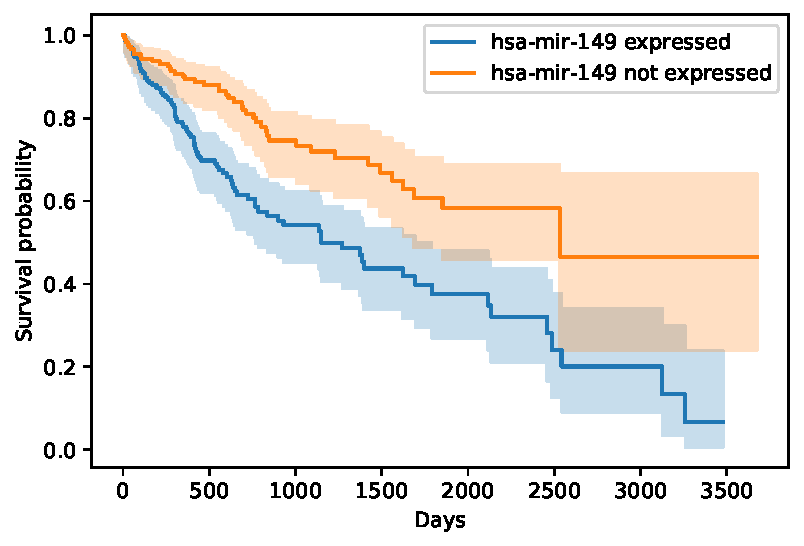
\includegraphics[width=0.48\textwidth]{hsa-mir-149}\hfill
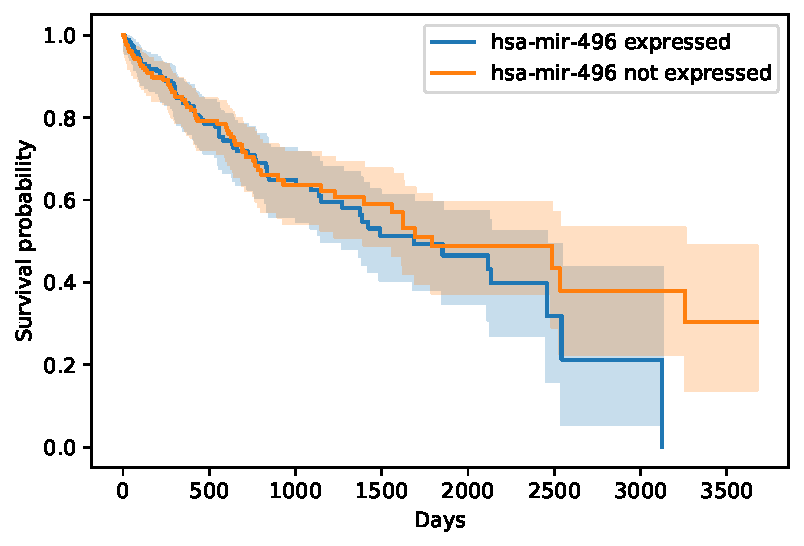
\includegraphics[width=0.48\textwidth]{hsa-mir-496}
\caption{\small\bold{Primer Kaplan-Meierjeve preživetvene krivulje za dve skupini, definirani z izražanjem genov.} Preživetje je bistveno večje pri skupini bolnikov z močno izraženimi
microRNA hsa-mir-149 (leva slika). Razlika pri mikroRNA hsa-mir-496 (desna slika) ni tako očitna. Lahko bi rekli, da je hsa-mir-149 torej boljši biomarker za preživetje. Pri odkrivanju biomarkerjev je ena od nalog razvrščanje genov glede na stopnjo ločevanja skupin z različnim preživetjem.}
\label{fig:km-marker}
\end{figure}

\bold{V idealnem primeru bi torej podatkovno odkritje novih biomarkerjev zahtevalo le podatke o preživetju z ustreznimi profili izražanja genov.} Algoritmi bi nato presejali vse gene in poiskali tiste, ki najbolje opredeljujejo skupine z različnimi funkcijami preživetja. Obstaja pa veliko težav in izzivov v tem postopku povezanih s šumom v podatkih, z majhnim številom preiskovanih vzorcev, z interakcijami med geni in vključevanjem razpoložljivega dodatnega znanja (podatkovnih baz). S tem se ukvarjamo podrobneje v nadaljevanju.

\subsubsection*{Predstavitev problema}

\bold{Predlagani projekt obravnava tri kategorije problemov in izzivov, ki vplivajo na
računske metode za ugotavljanje potencialnih biomarkerjev, pristopov k fuziji podatkov in izvedbe:}
\begin{description}
	\item[Računski izzivi, šum in prekomerno prilagajanje modela učni množici (ang.~{\em overfitting}).] Eksperimentalni podatki za preživetje, povezani z npr. vplivom novega zdravljenja ali zdravila, so pogosto dragi in zato so eksperimentalni vzorci majhni. V tipičnem kliničnem poskusu prve faze je pogosto manj kot 30 bolnikov, v 2. kliničnem poskusu pa je več kot sto bolnikov prej izjema kot pravilo. Podatkovni šum, povezan z načinom zbiranja, obdelavo vzorcev in merjenjem ekspresije genov, je lahko visok. Tako okolje lahko vodi do lažnih odkritij in prekomernega prilagajanja modela učni množici. Težava je še posebej očitna pri iskanju skupin ali mrež genov, ki bi lahko služili kot biomarkerji, saj število kandidatov (različnih skupin genov) raste eksponentno z želeno velikostjo nabora genov za biomarker. Na primer, za $20000$ genov, ki kodirajo beljakovine, obstaja več kot  $1.3$ bilijonov možnih genskih trojk. Tudi če bi nam uspelo vse računsko preučiti, bi to nujno povzročilo prekomerno prilagajanje modela učni množici, zato bi se rezultati dobro opisovali učne podatke, vendar bi se slabo posploševali na nove primere. Poleg šuma in prekomernega prilagajanja modela (ang.~{\em overfitting}) računski izzivi vključujejo še iskanje pragov ekspresije genov (kdaj je gen izražen?) in agregacijske funkcije (kdaj je skupek genov aktiven?).
 	\item[Vključevanje podatkovnih baz.] Geni sodelujejo v molekularnih poteh, funkcionalnih skupinah in odzivih na kemikalije in zdravila. Znanje o tem in druge genske anotacije so shranjene v podatkovnih bazah, kot so GeneOntology\myurl{http://geneontology.org}, KEGG\myurl{https://www.genome.jp/kegg}, CellMarker\myurl{http://biocc.hrbmu.edu.cn/CellMarker} in druge. Preučevanje genskih kompletov kot kandidatov za biomarkerje bi lahko in bi moralo uporabiti te dragocene vire informacij; tako za omejevanje prostora za iskanje biomarkerjev kot za razlago naborov najboljših kandidatnih genov (obogatitev genskega nabora). Takšno združevanje podatkov in baz znanja je že prineslo zanimive rezultate v bioinformatskih raziskavah~\cite{pmid30467459,pmid26465776}, vendar je bilo na področju odkrivanja biomarkerjev preživetja premalo raziskano.
 	\item[Vmesnik za raziskovanje podatkov.] V zadnjih dveh desetletjih so se pojavile različne metode, statistična orodja in orodja za strojno učenje za analizo visoko zmogljivih podatkov iz molekularne biologije. Analizi preživetja pa manjka elegantna zbirka orodij z intuitivnim uporabniškim vmesnikom, ki bi pomagala pri odkrivanju biomarkerjev, podpirala interaktivno analizo raziskovalnih podatkov v realnem času in ponudila enostavno izdelavo analitičnih podatkovnih cevovodov. Na voljo so dobre računalniške knjižnice za analizo preživetja v jezikih R in Python, vendar so to le nepovezani gradniki, ki za uporabo in integracijo zahtevajo napredne programersko znanje. Namesto tega končni uporabniki in znanstveniki s področja potrebujejo orodja za komunikacijo, raziskovanje in modeliranje podatkov ter intuitivna orodja s prilagodljivimi interaktivnimi vmesniki.
\end{description}

\bold{V projektu bomo te tri izzive napadli z razvojem novih tehnik in orodij za interaktivno raziskovanje potencialnih prognostičnih biomarkerjev.} Naš cilj je demokratizirati to področje z razvojem metod in interaktivnega vmesnika za inteligentno analizo podatkov preživetja.

\subsubsection*{Cilji projekta}

\bold{Projekt bo razvil in uporabil nabor računskih orodij za odkrivanje biomarkerjev iz podatkov genskega izražanja in kliničnega preživetja.} Vključili bomo obstoječe pristope k ocenjevanju biomarkerjev na podlagi podatkov o preživetju, modeliranje preživetja in analize obogatitve genskega nabora. Predlagali bomo tudi nove tehnike za analizo preživetja glede na specifične genske interakcije, za izdelavo omrežij markerskih genov in interpretacijo vizualizacij. Razvili bomo metode za hevrističnega iskanje, ki bo uporabljalo objavljene podatkovne baze o genskih funkcijah in presnovnih poteh.

\bold{Projekt bo opolnomočil domenske strokovnjake za uporabo teh orodij v resničnih aplikacijah, v realnem času in brez potrebe po pisanju računalniške kode.} Projekt bo vključeval računske metode v komponente z grafičnim uporabniškim vmesnikom. Izboljšali bomo lastno odprtokodno platformo za rudarjenje podatkov Orange\myurl{http://orangedatamining.com}~\cite{Demsar2013,Curk2005,Godec2019} (slika~\ref{fig:orange-workflow}) z novimi metodami za analizo preživetja. Pokazali bomo, da nastala platforma za vizualno programiranje ne samo bistveno zmanjša zapletenost in čas, porabljen za analizo podatkov, ampak tudi izboljša sodelovanje različnih strokovnjakov z informativnimi vizualizacijami in avtomatsko uporabo domenskega znanja.

\bold{Na koncu bomo predstavili še uporabnost izdelanega orodja.} Uporabili bomo nabor javnih in zasebnih (od sodelujočega podjetja Genialis) podatkov genske ekspresije in ustreznih kliničnih izidov. O uspešnosti projekta se bo presojalo glede na predstavljene primere uporabe in našo zmožnostjo, da nove uporabnike usposobimo za samostojno uporabo razvite tehnologije.

\begin{figure}[htbp]
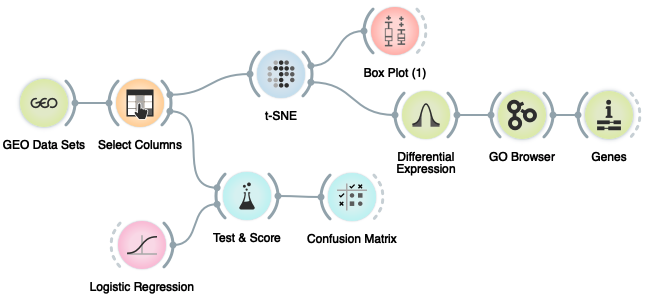
\includegraphics[width=0.7\textwidth]{orange-workflow}
\caption{\small\bold{Tipičen potek dela v programu Orange.} Slika prikazuje primer, ko smo ponovno analizirali gensko izražanje v mononuklearnih celicah periferne krvi. V raziskavi (GDS5363) so avtorji ugotavljali, ali je profiliranje ekspresije genov lahko zaznalo pojav osteoartritisa~\cite{Ramos2014}. Potek dela naloži podatke iz baze Gene Expression Omnibus in definira odvisne spremenljivke (stanje bolezni, izbrane komponente {\em Select Columns}). Zgornja veja postopka preveri strukturo vzorcev tkiva (komponenta {\em t-SNE}), za izbrane vzorce najde različno izražene gene in analizira njihove skupne značilnosti z obogatitvijo izrazov genske ontologije. V spodnji veji preverimo hipotezo preiskovalcev neposredno in ocenimo natančnost napovedi logističnega regresijskega modela s pomočjo navzkrižne validacije (komponenta {\em Test \& Score}). V predlaganem projektu bomo razvili podoben potek dela, vendar s komponentami, ki bodo naložile, obdelale, analizirale in prikazale podatke o preživetju ter predlagale nove biomarkerje.}
\label{fig:orange-workflow}
\end{figure}

\begin{figure}[htbp]
\floatbox[{\capbeside\thisfloatsetup{capbesideposition={right,top},
capbesidewidth=0.37\textwidth}}]{figure}[\FBwidth]
{\caption{\small\bold{Večina grafičnih komponent v programu Orange je interaktivnih.} Tukaj prikazujemo vsebino več komponent iz poteka dela v Sliki~\ref{fig:orange-workflow}. Uporabnik lahko na primer izbere podmnožico podatkovnih točk iz vizualizacije {\em t-SNE} (podatkovne točke z rumenim obrisom zgoraj desno) ali ustrezne podatke v  {\em Box Plot} ali nabor genov, ki so povezani z izbranim izrazom iz modula  {\em GO Browser}. V pripomočku  {\em Differential Expression} lahko izberemo nabor različno izraženih genov v repih porazdelitve. Večina modulov omogoča različne ravni interakcije in medsebojnega povezovanja. Projekt bo nekatere vizualizacijske komponente, vključno s {\em t-SNE}, ponovno uporabil in razvil specializirane, visoko interaktivne module za analizo preživetja in odkrivanje kompleksnih biomarkerjev.}
\label{fig:orange-interactivity}}
{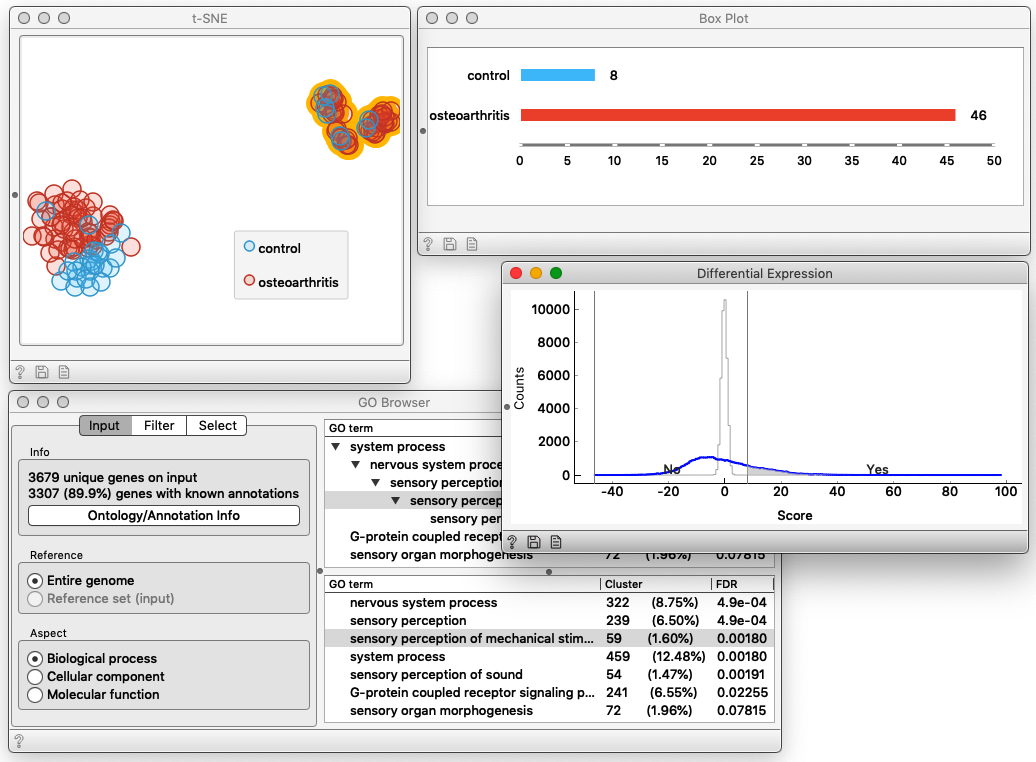
\includegraphics[width=0.6\textwidth]{orange-interactivity}}
\end{figure}

\subsubsection*{Pričakovani rezultati}
Najpomembnejši pričakovani rezultati tega projekta so:
\begin{enumerate}
	\item \bold{XXXXXXXXXXXXX New methods and approaches for biomarker discovery}, including computational approaches for survival-based biomarker interaction analysis, visualization approaches to map the space of potential biomarkers, and improved heuristic search for groups of biomarkers through the integration of data and knowledge-bases. XXXXXXXXXXXX
	\item \bold{Knjižnica računalniške kode z metodami za odkrivanje biomarkerjev iz podatkov o preživetju in genskem izražanju.} Knjižnica bo razvita v jeziku Python in bo objavljena v odprtokodni različici na GitHub skupaj z dokumentacijo, testi in primeri uporabe.
	\item \bold{Nabor orodij za odkrivanje biomarkerjev z vmesnikom za vizualno programiranje, interaktivnimi vizualizacijami in razlago rezultatov.} Nabor orodij bomo združili z javnimi podatkovnimi bazami in tako omogočili gradnjo analitičnih cevovodov v realnem času, in interaktivno vizualizacijo podatkov in modelov (glej sliko~\ref{fig:orange-interactivity}), podprto z domenskim znanjem.
	\item \bold{Nabor primerov uporabe, razvit v tesnem sodelovanju z Genialis.} Primeri uporabe bodo prikazali uporabnost naše programske opreme, moč intuitivnega grafičnega vmesnika in zagotoviti učno gradivo za razširjanje rezultatov projekta.
\end{enumerate}

% \subsubsection*{Our Preliminary Results and Studies}

% gene network discovery, gene interactions, intelligent data visualization, embedding, Orange.

\subsection{State-of-the-art in the proposed field of research and survey of the relevant literature}

The log-rank test and Cox's proportional hazards model are most commonly used in the literature to compare survival between two different groups of observers~\cite{singh2011survival}. These two methods can be regarded as a baseline to design strategies for detecting predictive marker genes. In a nutshell, the search for marker genes can be split into two subproblems: the grouping, or better, binarization of response variables (e.g., expression of the genes) and the search for promising predictive gene groups.

In clinical studies, biological markers are usually continuous variables obtained by various measurements. Establishing a cut-off point that represents the boundary between high and low gene expression, or more generally, that distinguishes between high and low risk groups, may be essential for their use in clinical decision making~\cite{mazumdar2000categorizing}. Budczies et al.~\cite{budczies2012cutoff} propose several approaches to selecting cut-off values: according to the distribution of the biological marker, by optimizing the interdependence of the target variable, such as response to treatment, or by finding a minimum p-value. The latter is the most common and selects the cut-off value according to the optimal difference in the survival outcome prediction between the groups~\cite{woo2020determination}. In general, however, finding the optimal value is a difficult problem that also depends on the study or research itself. Proper procedures to find the limit value are very important, as we may overestimate the true effect of the biological marker~\cite{Altman1991}.

Witten et al.~\cite{witten2010survival} highlight the problem of finding predictive features in high-dimensional data. When the number of variables is many times greater than the number of cases, the usual statistical approaches to survival analysis are no longer sufficient. There are many different published approaches to finding marker genes. Some recommend two-stage filtering: first, filtering differentially expressed genes (genes that distinguish well between selected groups), and then, further narrowing the set of possible candidates based on statistical significance in survival analysis~\cite{wang2017identification,liao2018identification,zhang2011discovery,kim2013identification}. Relator et al.~\cite{relator2018identifying} are critical of such approaches because they may leave many possible combinations of genes untested. They suggest a solution that can detect interactions of potential markers that conventional approaches would omit. An important shortcoming of their approach, as they acknowledge themselves, is computational complexity. They suggest splitting the data into smaller samples, running the proposed solution over the individual samples, and then combining the results. Consequently, also the proposed solution may omit promising gene interactions.

In complex diseases such as cancer, the effects of genomic data on survival are generally nonlinear. To detect nonlinear gene relationships, various approaches with deep learning techniques have emerged recently ~\cite{hao2019interpretable}. Several different models of deep learning have been proposed to predict survival, including the standard Cox model of relative risk (Cox-nnet~\cite{ching2018cox}, SurvivalNet~\cite {yousefi2017predicting}, DeepSurv~\cite{katzman2018deepsurv}). Despite advanced techniques and an increase in the number of potential biological markers, very few have been clinically used~\cite{burke2016predicting}. If the markers found are difficult to explain, insufficiently researched, or without known biological functions, they may be discarded despite their promise. With deep learning models, this challenge is all the greater. Hao et al.~\cite{hao2019interpretable} are taking a step towards finding explicable gene marker groups with deep neural networks by incorporating genomic and clinical data.


Besides computational methods, the proposed project will also relate to existing published applications of survival analysis. For example, Xiwen et al.~\cite{liao2018identification} and Wang et al.~\cite{33313167} studied correlations between miRNAs and the prognosis of hepatocellular carcinoma patients (HCC). They both established a five-miRNA signature model that could serve as a potential biomarker in the prognosis of HCC patients. Similarly, Guodong et al.~\cite{31799184} identified a novel five-miRNA signature model as a prognostic biomarker in colorectal cancer patients. Different approaches and methods were tested using miRNA expressions and related clinical data accessible through the TCGA database. Furthermore, Martinez-Ledesma et al.~\cite{26202601} explored the network-based approach and identified a gene expression-based biomarker that can successfully predict the clinical outcome of 12 different types of cancer. Listed studies are a great example of the importance of projects like TCGA. The comprehensive and structured data from the TCGA database may drastically speed-up the development of techniques for discovering (Di et al., \cite{29676997}) and validating (Chen et al.~\cite{32289666}) promising gene-based biomarkers.


% \subsubsection*{Computation Methods for Gene Markers Identification in Survival Analysis}
% \subsubsection*{Visual Data Analysis}
% \subsubsection*{Toolboxes}

\subsection{Detailed Description of the Work Programme}

\subsubsection{Project Tasks}

The project will be organized around the following set of tasks:
\begin{description}
	\item[T0] \bold{Setting-up of the collaborative environment.} We will deposit all the code and documentation on GitHub\myurl{https://github.com/biolab}. The repository will store project documentation and meeting minutes, tasks management through creation and tracking of issues, Python library code, unit-test, and examples. Data files will be stored on a separate web server. Extensions of Orange\myurl{https://orangedatamining.com} will be developed as an add-on and will be stored in a separate repository on the GitHub.
	\item[T1] \bold{Data acquisition and organization.} The project will use a number of different data sets coming from published studies and databases such as NCBI's Gene Expression Omnibus\myurl{https://www.ncbi.nlm.nih.gov/geo} and TCGA, The Cancer Genome Atlas database\myurl{https://portal.gdc.cancer.gov}. In addition, we will also create a set of synthetic data sets of varying size and complexity. The compiled data sets will be stored on Genialis Expressions\myurl{https://www.genialis.com/software-applications/}, an online database of gene expression and other biomedical data, provided by Genialis.
	\item[T2] \bold{Development of data mining and bioinformatics for survival biomarker discovery.} In particular, we will develop and implement techniques for:
	\begin{description}
		\item[T2.1] \bold{Gene ranking and selection based on the survival function}, where we will implement standard techniques from the field, including the log rank test and the ranking based on the inference of Cox proportional hazards model. We will also include more recent and advanced modeling approaches based on random forests and deep learning, and infer gene ranking through studying the sensitivity of the models.
		\item[T2.2] \bold{Feature construction}, where we will use predictive models on a smaller subset of genes to aggregate gene expression and with this aim to increase the robustness of so-inferred biomarker. We will employ $\ell 1$ regularization in combination with Cox and derived models, and network-based approaches where biomarker is composed of a small number of genes from the same regulatory network or metabolic pathway.
		\item[T2.3] \bold{Gene interaction analysis}, where we expect that a group of genes can interact in a non-linear way to form a more robust and informative biomarker. We will adapt the approaches for finding feature interactions to address survival data, and the approaches to visualize the results of interaction analysis.
		\item[T2.4] \bold{Knowledge-infused biomarker discovery}, where we will restrict the search space of survival-effecting gene interactions to groups of genes with shared functional annotations from knowledge libraries on gene annotations, pathways, established panels for measuring gene expression (e.g. nanoString) and known markers.
 		\item[T2.5] \bold{Deep and transfer learning}, where our aim is to find gene embeddings for their profiling in low-dimensional space. We will use auxiliary dataset to train (tissue-specific, disease-specific) variational autoencoders~\cite{doersch2021tutorial} for embedding, and then adapt the embedding to specific survival problem using transfer learning~\cite{Godec2019}, that is, modifying only a small part of the deep model. We will use the embedded, latent profiles of genes for visualizations of gene maps and in heuristics to restrict the search space.
 		\item[T2.6] \bold{Gene interaction maps}, where we would like to represent genes---potential biomarkers---in a gene map where vicinity of genes on the map suggest increased joint effect on the survival function. Building on the knowledge and tools for co-expression analysis, these constructed interaction plots will serve for mapping of interaction space and presentation of the space of solutions to biomarker discovery problem.
		\item[T2.7] \bold{Automatic annotation of point-based visualizations}, where points are genes and a primary example of such visualizations are gene interaction maps. We will devise algorithms that search for visualization neighborhoods with enriched gene function or pathways, and annotate visualizations accordingly. This research will follow our prior work on annotation of gene maps for single-cell analysis~(see Fig.~\ref{fig:annotation}).
	\end{description}
	\item[T3] \bold{Design of visual interfaces for exploratory analysis of survival data and biomarker discovery.} In a close collaboration with the partnering SME, we will lead a thorough requirements analysis and product discovery process that will ensure a proper design of components and pipelines for interactive, domain-knowledge driven mining of biomarkers from survival-related gene expression data. The design will include the planning of a set of computational components to address all aspects of survival analysis and biomarker discovery. We will design the graphical interface of the components, their visual presentation, interactive visualizations, and possible data analysis pipelines to combine the design components. The deliverable will include sketches of graphical user interface (in Balsamiq Mockups) and wire-frames. The design will emphasize the quality of user experience, access to advanced computational techniques, and ability to combine components in a Lego-brick way to devise possibly complex and powerful analysis pipelines.
 	\item[T4] \bold{Implementation and Integration.} The developed computational techniques will be implemented within the open-source data mining environment Orange\myurl{http://orangedatamining.com}. The implementation will use the library of methods from task T2 and graphical user designs from T3. Implementations will be released as an separate add-on to Orange, and will follow implementation guidelines which refer to documentation, and unit testing with near 100\% code coverage.
 	\item[T5] \bold{Experimental evaluation.} The developed functionality will be be thoroughly tested in collaboration with Genialis, our project partner. Synthetic and real data sets (prepared under Task 1) will be used, and results compared to those from the literature. The validation will confirm the validity and correctness of developed procedures and will serve to collect case studies to be published on GitHub, Orange's web site, and in planned publications and possibly patents.
 	\item[T6] \bold{Dissemination of results.} This task includes publishing of the implementation of the developed methods under General Public License (GPL), writing and web-publishing of relevant documentation with working examples, publishing video tutorials with use cases on Orange's YouTube channel\myurl{http://youtube.com/orangedatamining}, and dissemination in terms of presentation at relevant conferences and journal publications. We will target bioinformatics journals, such as {\em Bioinformatics}, {\em Nature Methods}, and {\em Artificial Intelligence in Medicine}, and related conferences, including the top-rated AIM and ISMB. Also, we are planning to file a joint patent with Genialis in the field of prognostic biomarker discovery.
\end{description}


\begin{figure}
\floatbox[{\capbeside\thisfloatsetup{capbesideposition={right,top},
capbesidewidth=0.37\textwidth}}]{figure}[\FBwidth]
{\caption{\small\bold{A prototype of Orange's widget with automatic annotation of point-based visualisation.} On the input, this component considers gene expression profiles of single cells and their associated embedding (e.g., t-SNE coordinates), and a list of marker genes for each candidate cell-type. In scope of the proposed project, we will use a similar approach to design a widget that would annotate and thus explain the space of potential markers.}
\label{fig:annotation}}
{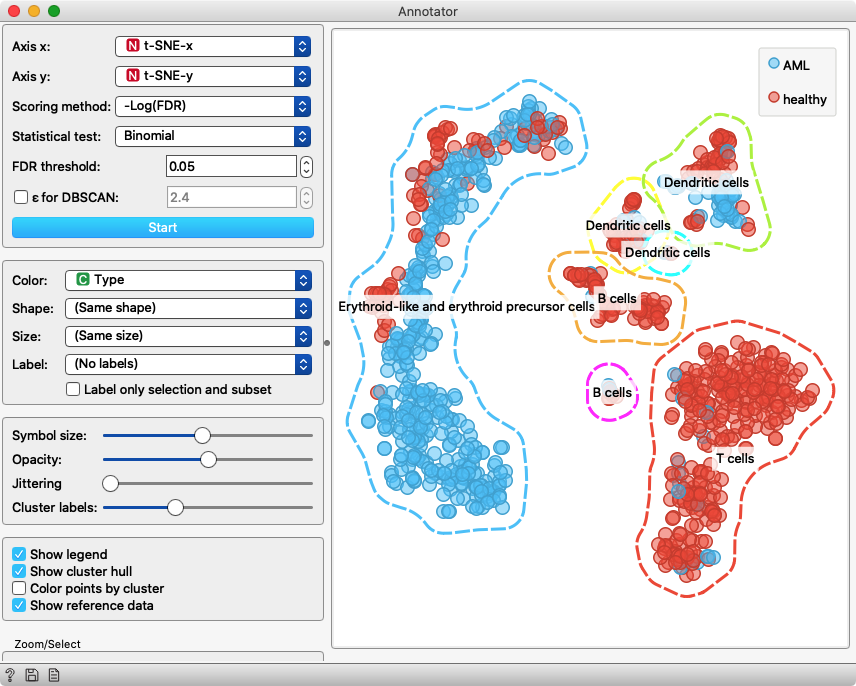
\includegraphics[width=0.6\textwidth]{annotation}}
\end{figure}

\subsubsection{Research Design and Methods}
\begin{description}
	\item[Overview.]
The overview of the research in the proposed project is presented in Fig.~\ref{fig:approach}. The figure shows how we will integrate the target gene expression data and clinical metadata with additional knowledge bases and other available data sets. It exposes the key scientific approaches we will address:
\begin{enumerate}
\item which, on their own, are the key molecular markers for survival,
\item which are the combinations of molecular entities (gene sets) that jointly correlate with survival,
\item which characteristics of marker genes can help us interpret the results of the analysis.
\end{enumerate}
While all of the above are clearly the issues that could be individually and manually addressed by a molecular biologist, due to the sheer volume of data and additional information in available data and knowledge bases they can only be tackled through means of computational analysis and data-driven approaches. The principal challenge of the project is how to combine these different sources, and use modern data mining approaches to support knowledge discovery to provide interpretable and operational hypotheses to biomedical researchers and drug developers. In the description below, we first list the data sources on which we will apply our marker discovery process, then list a set of computational approaches which we will develop and use, and comment on the feasibility of their implementation within the existing visual programming-based data mining framework.

\begin{figure}
\floatbox[{\capbeside\thisfloatsetup{capbesideposition={right,top},
capbesidewidth=0.37\textwidth}}]{figure}[\FBwidth]
{\caption{\small\bold{Knowledge-based analysis to biomarker discovery.} We aim to combine our target data set with transcription and survival data from clinical trials with other available data sets and knowledge bases to gain in speed, accuracy and interpretation of results. Substantial part of our project deals with exploratory data interfaces, which combine visualization of data, identified biomarkers and models. Together, computational approaches for biomarker discovery and visualization approaches for making these findings explicit and placing them in the context of entire search space (e.g., {\em marker maps}) will assist us in explainable, semi-automatic discovery process. The methods will provide hypotheses to be evaluated by a domain expert, and they will be able to work with the assumptions and curated public knowledge rather than machine-generated black-box decisions.}
\label{fig:approach}}
{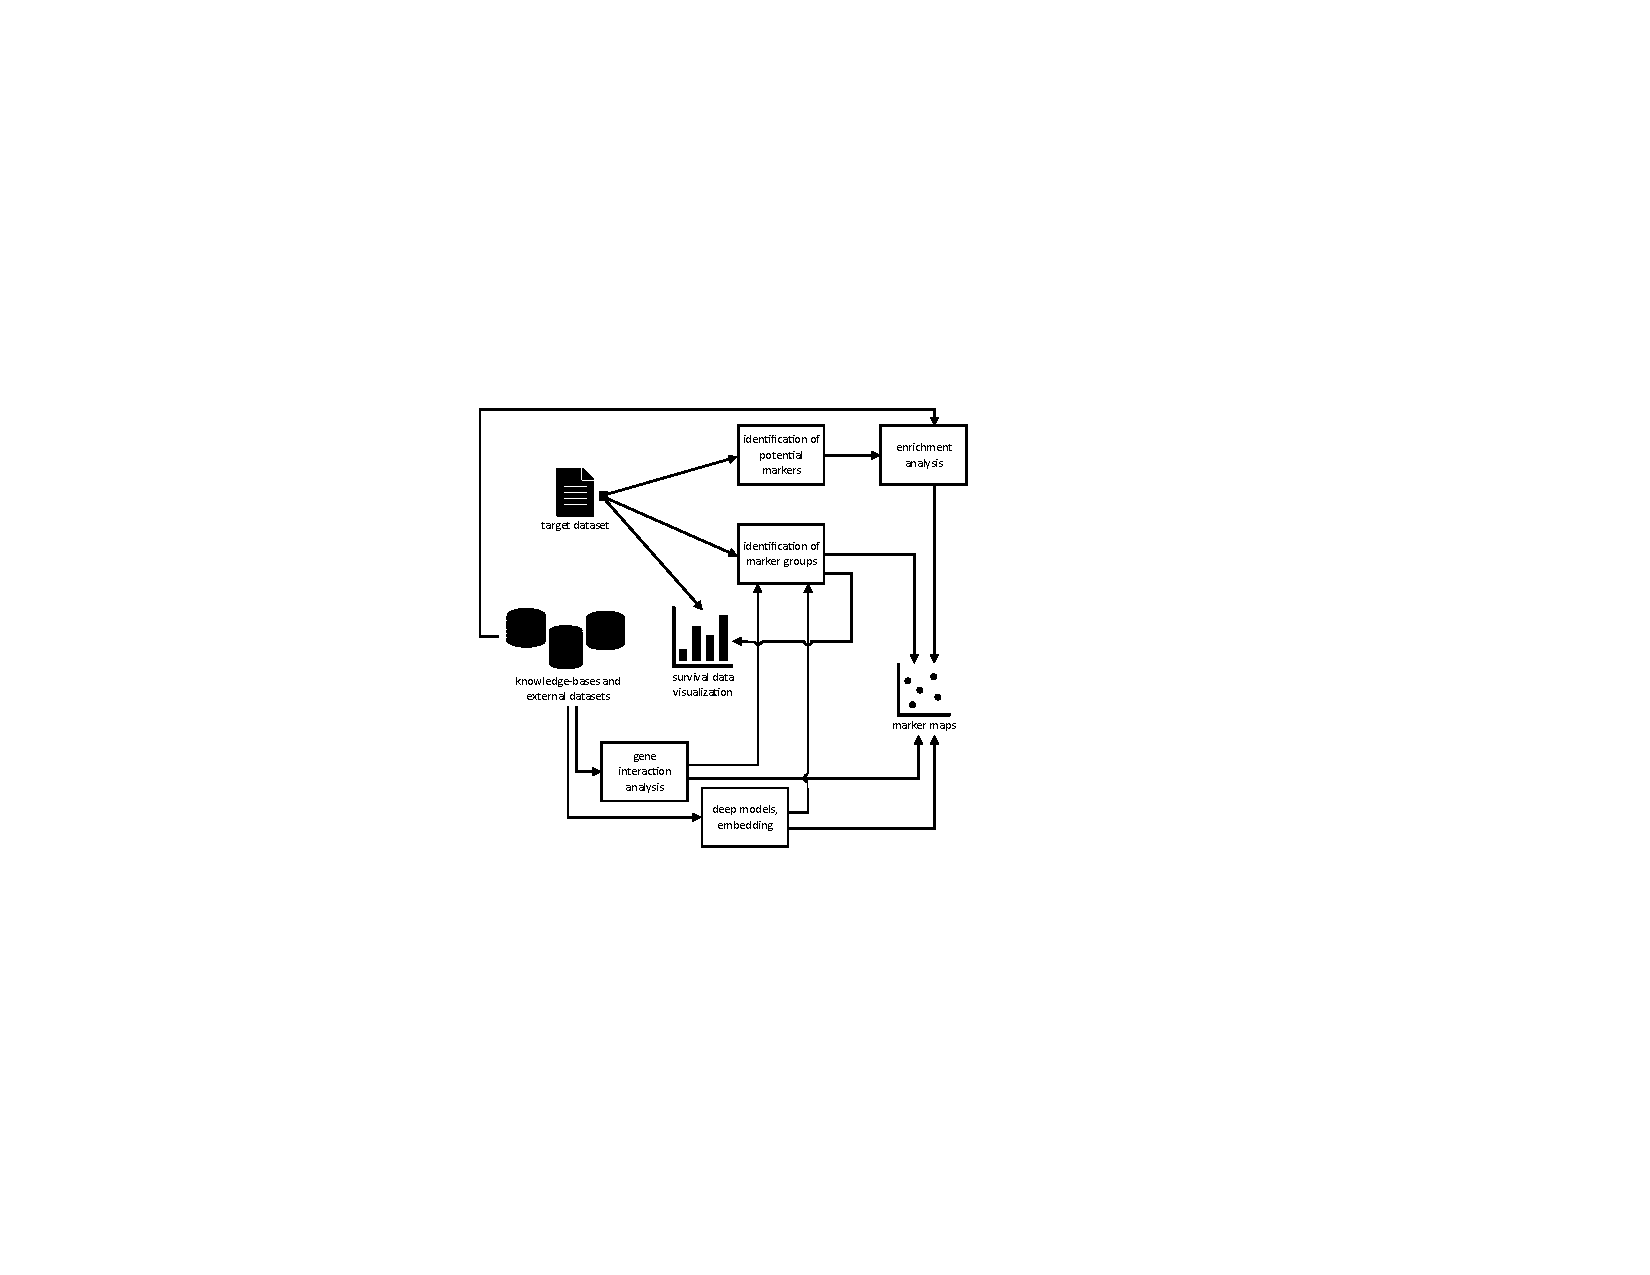
\includegraphics[width=0.6\textwidth]{approach}}
\end{figure}


% \begin{figure}
% 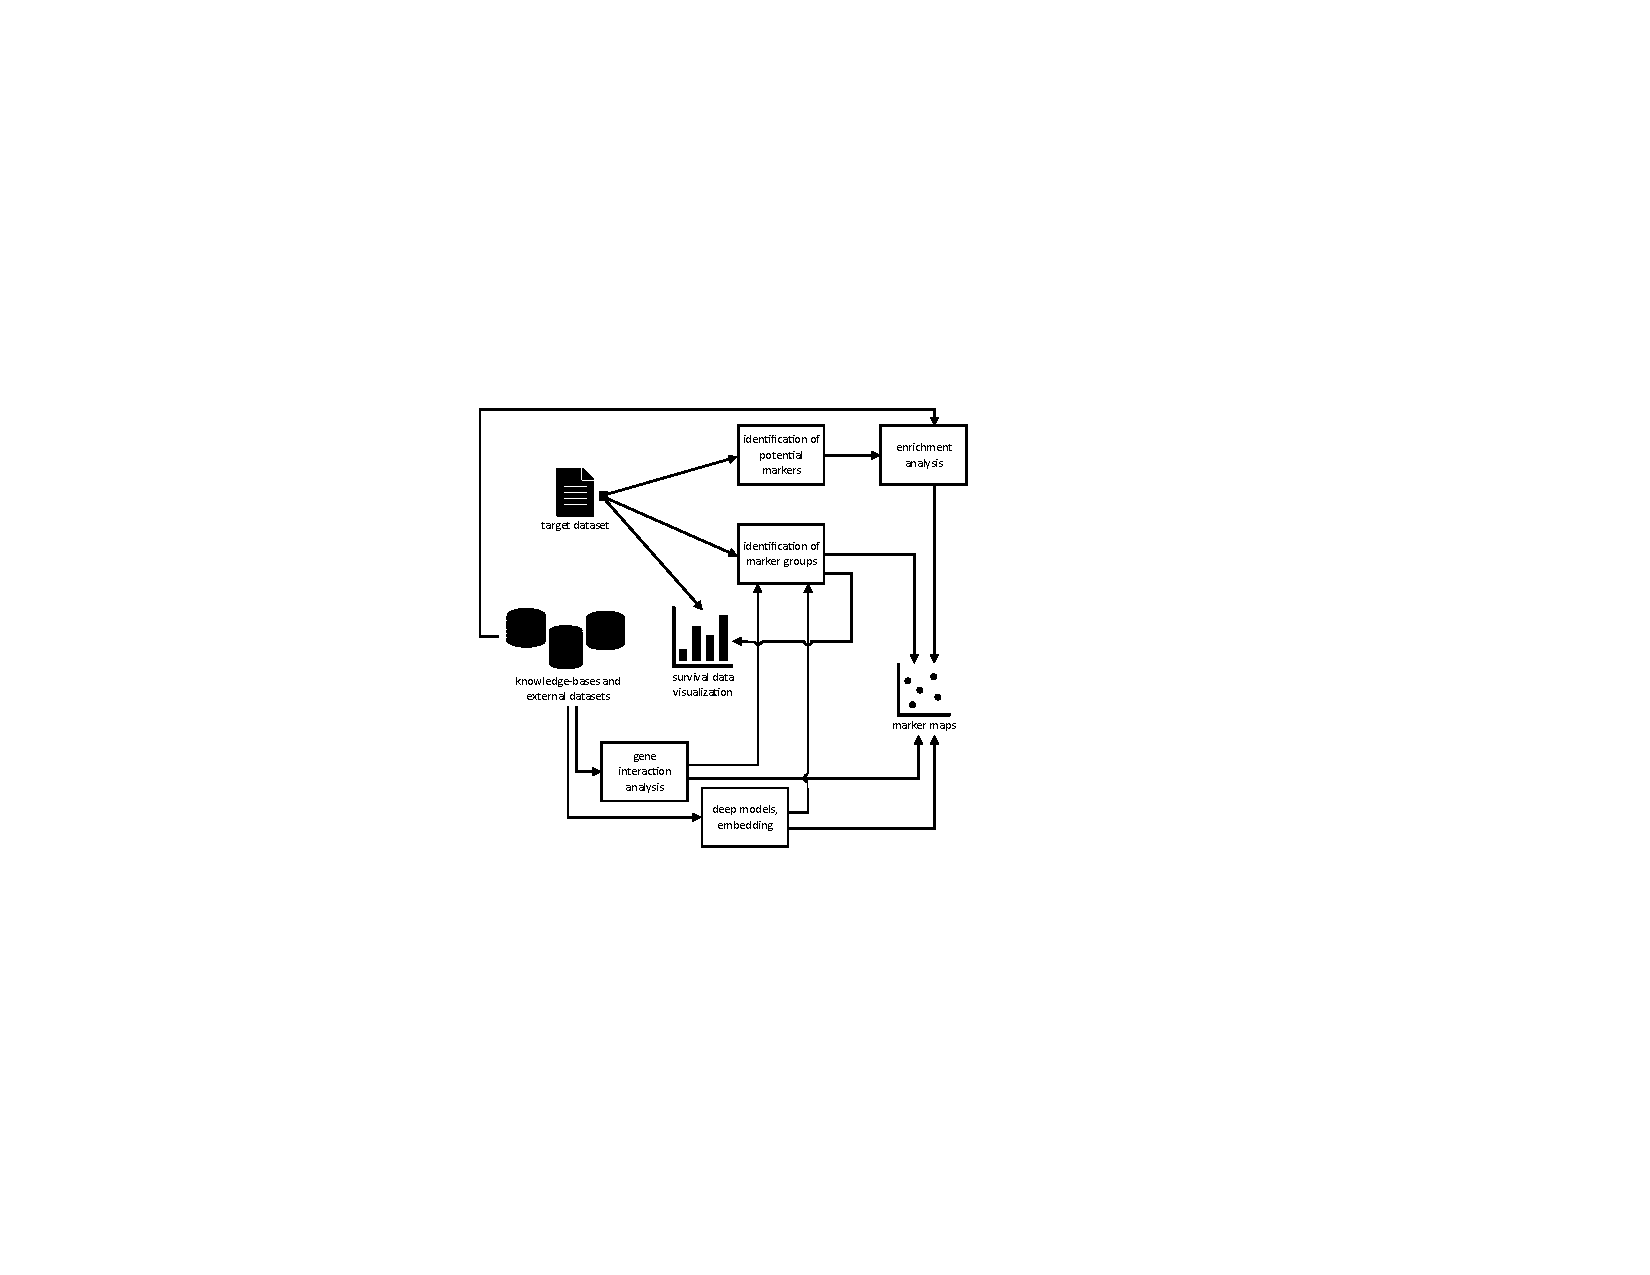
\includegraphics[width=0.48\textwidth]{approach}
% \caption{An example of a Kaplan-Meier plot for two gene expression-dependent conditions associated with patient survival. In panel a), the survival function is substantially higher for a group of patients with highly expressed microRNA hsa-mir-149. The difference is not so evident in the panel b) and microRNA hsa-mir-496. We could say that hsa-mir-149 is hence a better biomarker for survival. In biomarker discovery, one of the tasks is to rank genes and RNA molecules according to the degree of separation between corresponding survival signatures when a gene is expressed and not expressed.}
% \label{fig:approach}
% \end{figure}


	\item[Material and Data Sets.] Four types of data sets will be gathered, organized and used in the project:
	\begin{description}
		\item[DS1] Transcription data from The Cancer Genome Atlas database\myurl{https://www.cancer.gov/tcga}~\cite{24071849} and Gene Expression Omnibus\myurl{https://www.ncbi.nlm.nih.gov/geo/}~\cite{23193258}.
		\item[DS2] Survival analysis data from clinical trials from The Cancer Genome Atlas database.
		\item[DS3] Transcription and clinical trial data managed by Genialis.
		\item[DS4] Simulated data sets.
	\end{description}
	The data from DS1 and DS2 are fragmented; datasets have to be integrated, so that the clinical trial data is aligned with a corresponding transcription data. Methodological reports on development of computational techniques, including those we have cited in the related work, would refer to data repositories but would seldom publish the reorganized data ready to be used in off-the-shelf software packages. Our project aims to break with this practice and compile a data repository with aligned clinical and transcription data sets ready for benchmarking and comparing biomarker discovery techniques.

	Genialis d.o.o.~already has a collection of such align datasets which comes from their existing partnerships with some major pharmaceutical companies. The data is private, but will be shared with us in the project for testing and validation purposes.

	We will also construct a set of simulated datasets, where variables representing biomarkers will be placed by design. The datasets will serve for testing and benchmarking of the proposed methods.

	The project will additionally use other sources of information, which, for the reasons of convenience, will be queried for information specific for the project and will internally be represented as additional data sets. These include, but are not limited to:

	\begin{description}
		\item[DS6] Gene function annotations from Gene Ontology (GO) consortium.\myurl{https://www.geneontology.org}
		\item[DS7] Various pathways from KEGG, Kyoto Encyclopedia of Genes and Genomes.\myurl{https://www.genome.jp/kegg}
		\item[DS8] NDEx pathway data base.\myurl{http://www.ndexbio.org/}
		\item[DS9] Various marker gene data bases, including CellMarker\myurl{http://biocc.hrbmu.edu.cn/CellMarker}~\cite{cellmarker} and PanglaoDB
		\myurl{https://panglaodb.se}~\cite{30951143}.
	\end{description}

	\item[Computational Approaches, Data Mining and Bioinformatics.] Computational approaches and development of data mining methods will include:
	\begin{description}
		\item[Data organization (task T1).] The project will develop a computational platform with access to the common, server-based databases that will store transcriptome and survival data from third parties and participating SME Genialis. We will use standard software engineering practices to construct this architecture (data server with secure HTTP access, HTTP-based queries, components on clients to access the data). We will locally store the data from other information sources like gene ontologies and pathways to allow for fast computation and utility of such information, and for these reuse existing server and database architecture of Orange~\cite{Demsar2013,Curk2005,Godec2019}. Overall, the software engineering task here is to hide the details of data access and query from the user. Users should be able to access these functions with a single click and focus on data analysis and interpretation.
		\item[Gene ranking (T2.1).] We will use the standard log-rank test to compare two or more survival curves and hence estimate a selection of gene and its expression threshold to break observed cases to subpopulation. The log-rank test will be used as a baseline. We will compare the inferred ranking of genes to modeling approaches, where we will infer survival models first, and then estimate the information value of its constituents (genes) either directly for linear models (e.g.~Cox proportional hazards models) or indirectly. Advanced models will include random survival forests~\cite{22088987} and deep learning~\cite{katzman2018deepsurv,ching2018cox}. Indirect measurements of contributions of individual features will include game theoretic approaches such as SHAP\myurl{https://github.com/slundberg/shap}~\cite{32607472}.
		\item[Gene set enrichment analysis (part of T2.1).] We will use the gene set enrichment analysis~\cite{1239896} to interpret the results of the biomarker ranking and inspect commonalities of the best-ranked genes in terms of functions and pathways.
		\item[Feature construction and gene set identification (task T2.2).] We will use direct and indirect feature selection techniques.  The quality of the set will be estimated through the predictive performance of the model. As an alternative approach, we will use model-based feature selection, like $\ell 1$ regularization of Cox and network models.
		\item[Gene interaction analysis (T2.3)] will examine possible combinations of genes for their combined effect on the survival function. We plan to use model-based evaluation of gene pairs (T2.1) and represent results in interaction maps (T2.6) and networks.
		\item[Knowledge-infused biomarker discovery (T2.4)] will limit the search for useful combinations of features in task T2.2 to genes with common functional or pathway labels, that is, preferably to those already associated with investigated pathology in the literature. The success of this approach will be measured through gains in algorithm speed and reduction of search space to be considered, while requesting identification of the gene sets of similar quality to those from exhaustive search.
		\item[Deep learning (T2.5)] will employ variational autoencoders for embedding to represent marker candidates with latent vectors, that is, position them in the latent space where we can easily examine their relatedness and the structure of marker space. We will construct autoencoders from the gathered collection of transcription data and clinical data sets (task T1) and then use transfer learning~\cite{Godec2019} to adapt the model to a specific target dataset. The embedded representations of potential markers will provide the foundation to construct interpretable visualizations of the search space (e.g., task T2.6).
		\item[Gene interactions maps (T2.6)] will render information from tasks T2.3 and T2.7 and provide means for graphical explanation and presentation of the search space, exploratory data analysis, and visual interpretation. To render gene maps we will use our own variant of t-SNE~\cite{vanDerMaaten2008} called openTSNE\myurl{https://github.com/pavlin-policar/openTSNE}~\cite{policar2019}, which can preserve global structure.
		\item[Annotation of point-based visualizations] will equip gene maps (task T2.6) and other point-based visualizations of gene and marker search space with functional and pathway labels. We will use this approach to provide assisted interpretation of the search space. To develop this technique, we will extend our approach previously developed for single-cell gene expression analysis (see Fig.~\ref{fig:annotation}).
	\end{description}

	\item[Software Implementation.] Over the past two decades, we have been developing a comprehensive data analysis suite called Orange\myurl{https://orangedatamining.com}~\cite{Demsar2013,Curk2005,Godec2019}. Orange has been used by thousands of users and is a toolbox of choice in training of data science in hundreds of universities\myurl{https://orangedatamining.com/blog/2021/2021-01-11-orange-in-classroom/}. Orange features a scripting and a visual programming environment. Visual programming offers an intuitive means of combining known analysis and visualization methods into powerful applications. Orange includes a set of visual components for functional genomics (Fig.~\ref{fig:orange-interactivity}) that enable users who are not programmers to analyse transcriptomic data and to customize their analysis by combining common data analysis tools to fit their needs~\cite{Godec2019}. Orange framework will be used to implement methods proposed in this project and offer them to the community within an open-source model.

	Within the project, we will develop a set of components that will be specific to the problem in our project, but also general enough for other survival analysis tasks. We intend to develop components for survival modeling, accuracy estimation, biomarker ranking, identification of groups of markers, gene embedding, and construction of survival-based gene interaction maps. Orange includes components crucial for the proposed project but have already been developed or at least prototyped. These include access to gene annotation libraries, gene set enrichment, GO browser, and visualization tools, including t-SNE and Kaplan-Meier curves.

	\item[Experimental Validation.] We will use the data sets DS1 to DS4 to experimentally validate both the computational techniques and the visual interfaces we will construct in the project. There are three aspects of validation we will assess:
	\begin{itemize}
		\item \bold{predictive performance}, where we will compare inferred biomarkers to those published in the literature, and compare the results of our marker discovery techniques to those already published;
		\item \bold{interpretability}, which will be assessed with domain experts working with Genialis, a participating SME. The assessment of interpretability will be both quantitative, in terms of how well can we link identified biomarkers to known functional and pathway labels, and subjective, in terms of agreement of domain experts with the proposed result;
		\item \bold{usability}, where we will use hands-on workshops with domain experts to assess if they can use the developed tool independently after a three-hour training.
	\end{itemize}
\end{description}

\subsection{Available research equipment over 5.000 €}

Genialis, the participating SME, will provide a web resource Genialis Expressions (see Fig.~\ref{fig:genialis-expressions-frontend} and~\ref{fig:genialis-expressions-software-components}) to aggregate, curate, and analyze high-throughput sequencing data and associated clinical and experimental results. Genialis Expressions run on the AWS Kubernetes Cluster owned by Genialis.

\begin{figure}[htbp]
\floatbox[{\capbeside\thisfloatsetup{capbesideposition={right,top},
capbesidewidth=0.24\textwidth}}]{figure}[\FBwidth]
{\caption{\small\bold{Genialis Expressions} is a biomedical data hub that ensures FAIR (Findable, Accessible, Interoperable and Re-usable) guiding principles for scientific data management and stewardship. It automates primary analysis (pre-processing) of the next generation sequencing data and ensures data provenance and reproducability. Genialis Expressions facilitate collaboration, data sharing, and supports integration with 3rd-party apps like Orange.}
\label{fig:genialis-expressions-frontend}}
{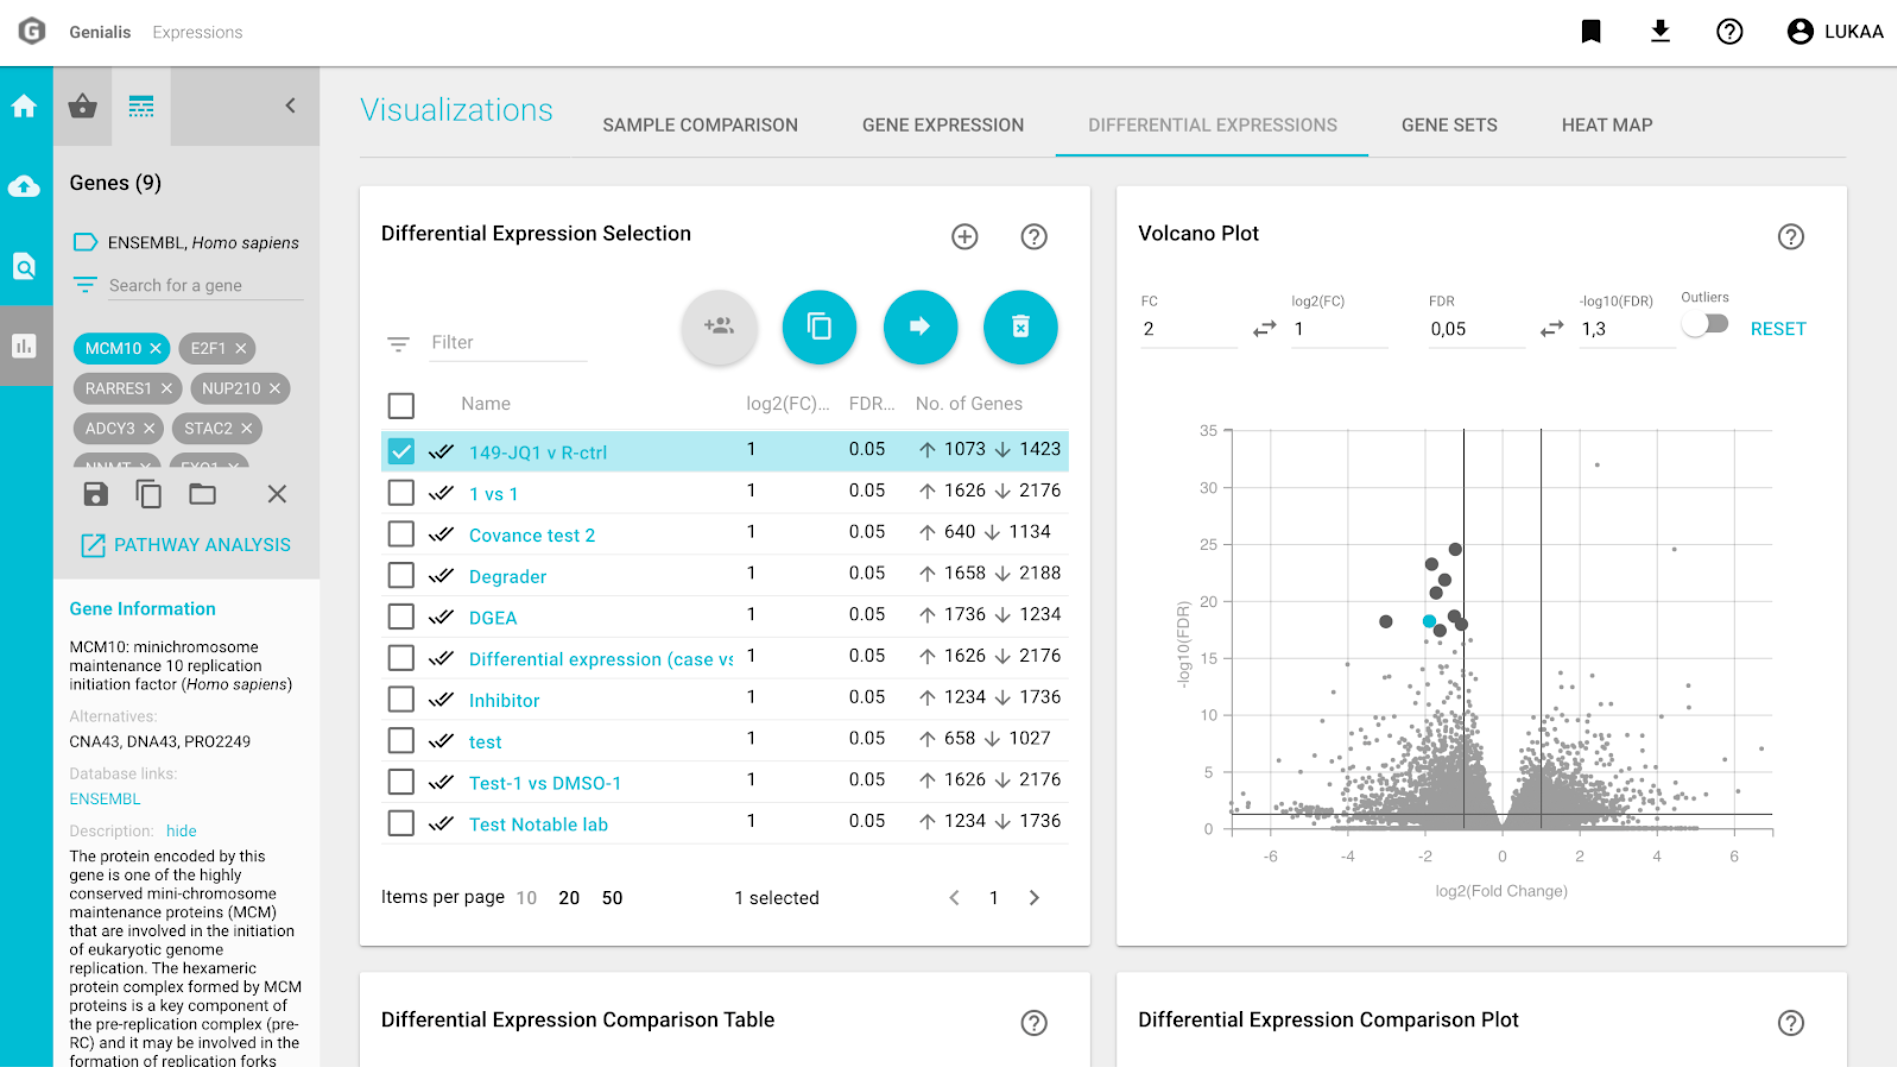
\includegraphics[width=0.73\textwidth]{genialis-expressions-frontend}}
\end{figure}

\begin{figure}[htbp]
\floatbox[{\capbeside\thisfloatsetup{capbesideposition={right,top},
capbesidewidth=0.2\textwidth}}]{figure}[\FBwidth]
{\caption{\small\bold{Modular software architecture of Genialis Expressions.} The frontend layer communicates with the backend via RESTful API. We provide TypeScript and Python software development kits (SDK) for integration with our proprietary frontend and 3rd-part software solutions, such as Orange (see the grey box in the top right corner). We support a plun-in architecture for analysis tools (see the brown boxes to the right). The analytics jobs run in parallel on the Kubernetes Cluster, each in its own isolated envrinment using Docker containers.}
\label{fig:genialis-expressions-software-components}}
{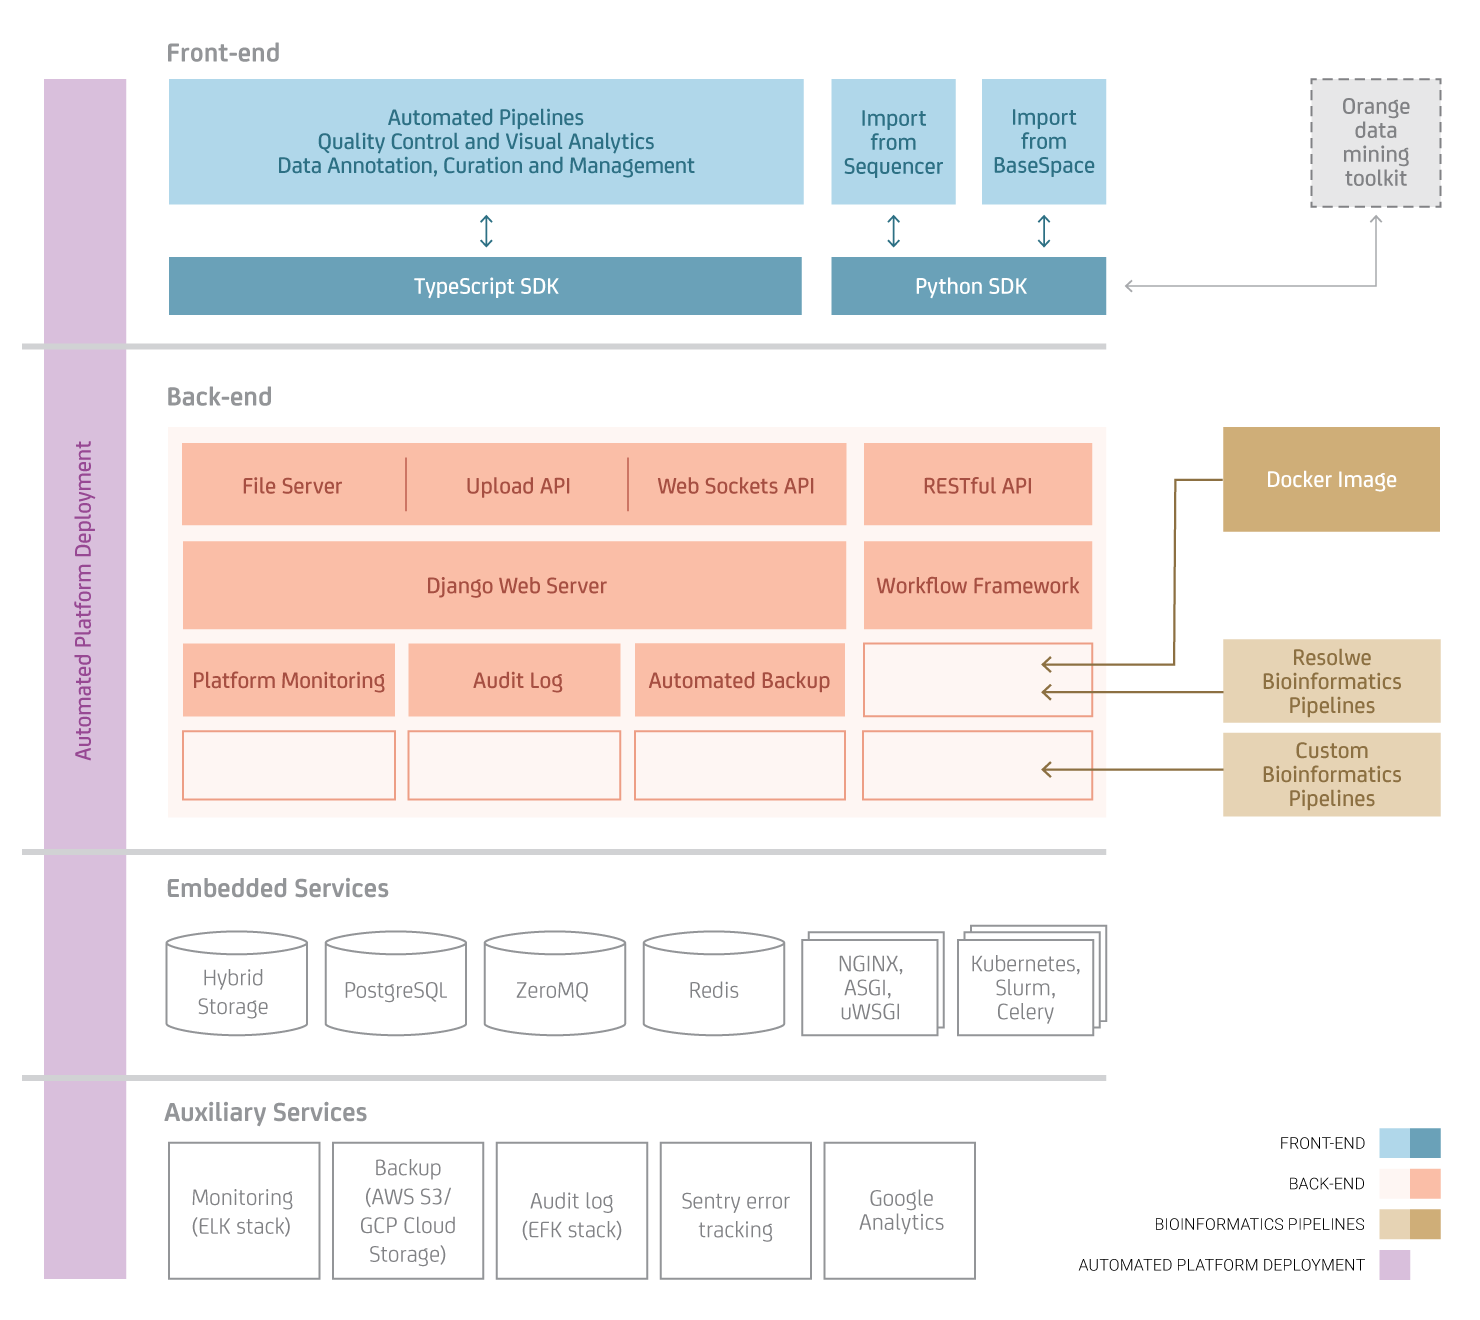
\includegraphics[width=0.8\textwidth]{genialis-expressions-software-components}}
\end{figure}

The project will use the computational infrastructure of Bioinformatics Laboratory of University of Ljubljana, which includes CPU cluster (about 500 processors), NFS storage (about 500 TB), and a cluster of GPU processors (about 20 GPUs), collectively valued at about 200.000 EUR. We will require no special computational equipment besides the existing for the proposed project.

\subsection{Project management}

The project will join two highly compatible R\&D teams. The Bioinformatics Laboratory from University of Ljubljana will bring to the project its extensive expertise in data mining, machine learning, bioinformatics, and computational phenotyping. The project will be co-financed by Genialis, a data science and drug discovery company focused on new ways to treat disease. Blending computational biology and AI-based methods, Genialis merges and models data at the intersection of clinical and translational medicine. Genialis is trusted by biopharma and big pharma alike, to validate targets, predict biomarkers and optimally position novel drugs. Together, Genialis and its partners are bringing improved solutions to drug discovery to change people's lives.

The project will be managed by UL (project manager). The management of the project will be organized through regular meetings of the management board, with one appointed representative from each institution, and through regular meetings of the project members. The collaboration platform will be based on GitHub and will be made available in the earliest stage of the project.

We will complete the project in three years. Fig.~\ref{fig:gantt} gives the detailed time line of the projects.

\begin{figure}
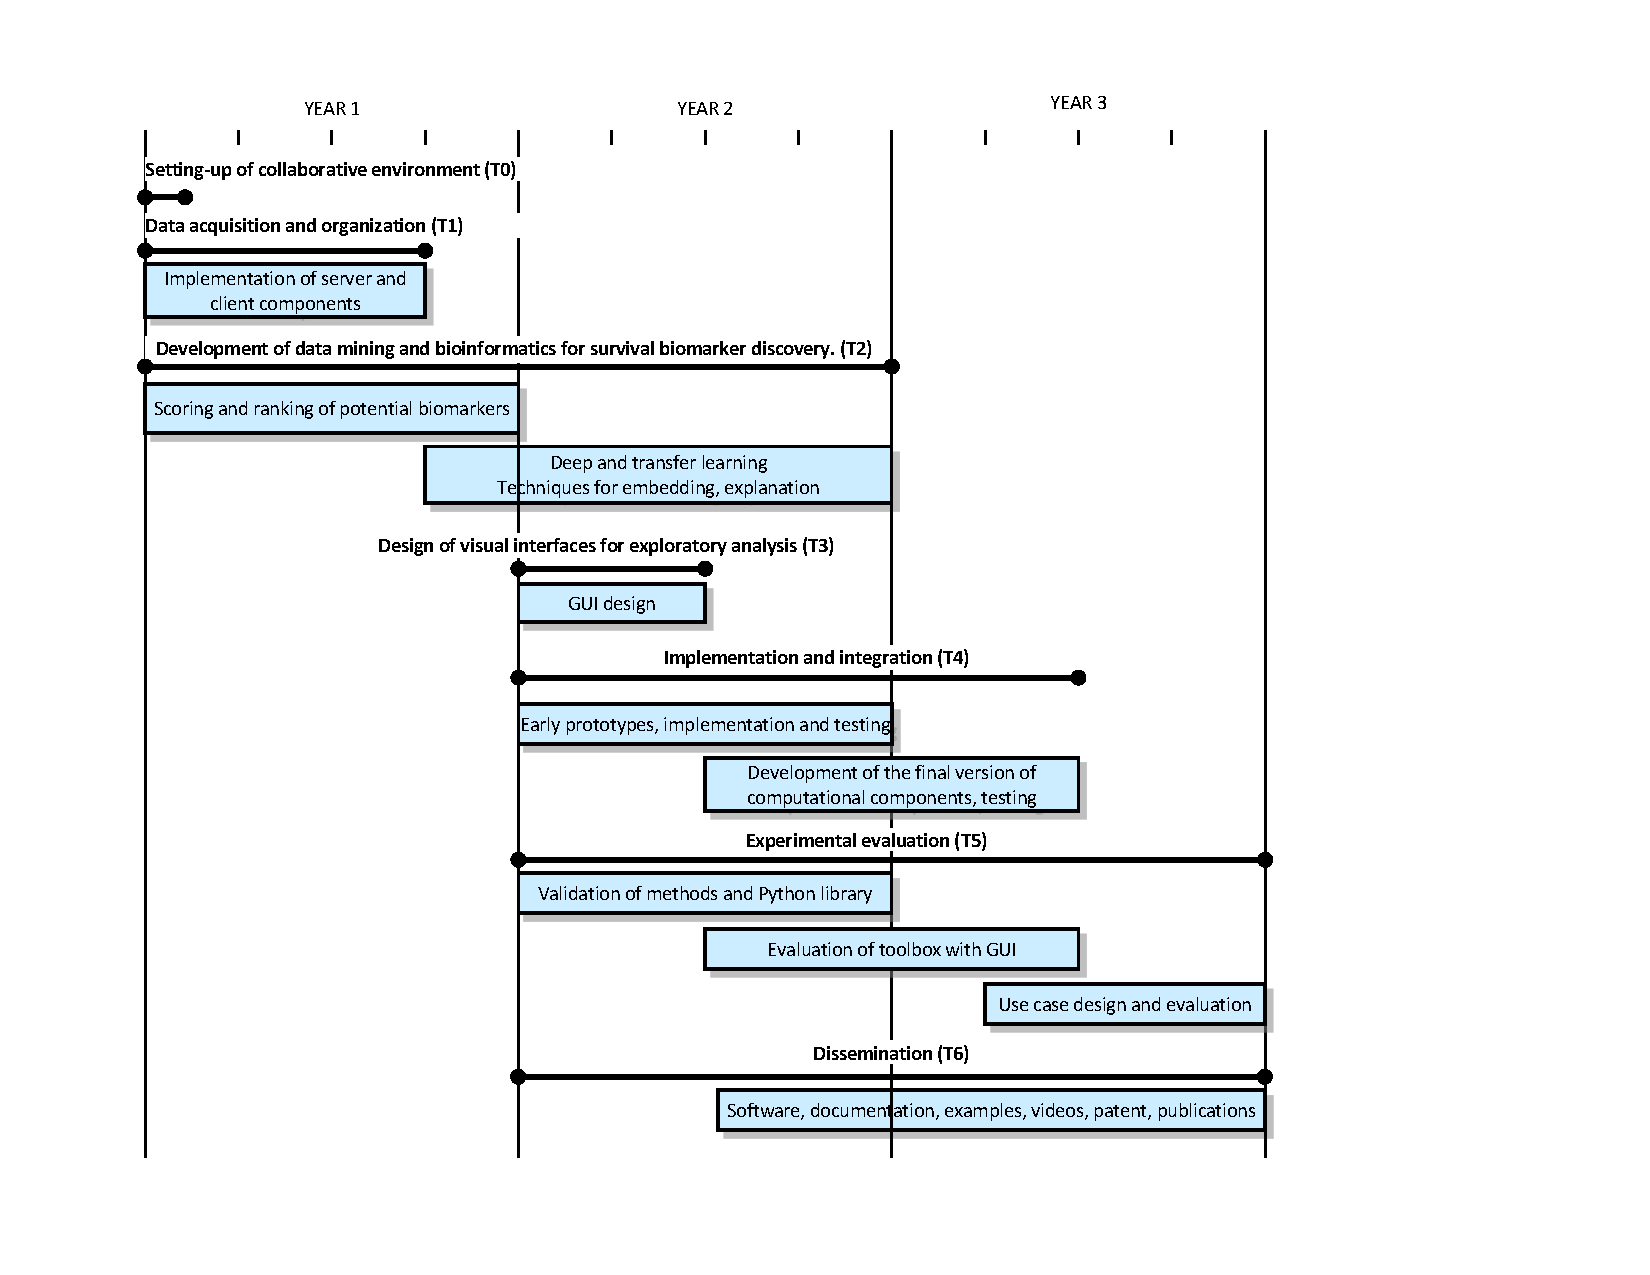
\includegraphics[width=0.90\textwidth]{gantt}
\caption{\small\bold{Project's time line}. In a nutshell, we will start with organizing the data sets. Then, we will develop a Python library for marker discovery in survival analysis. We will proceed with the design and implementation of the graphical user interface for new components of Orange data mining library. All components of the developed system will be tested in collaboration with Genialis, our partner SME. A special task is devoted to dissemination, which includes open-source software, documentation, examples, video material, scientific publications, and filing of a patent.}
\label{fig:gantt}
\end{figure}

% \clearpage
\subsection*{References}

\patchcmd{\thebibliography}{\section*{\refname}}{}{}{}

\begin{multicols}{2}
\footnotesize
\setlength{\parskip}{0em}
\renewcommand{\baselinestretch}{1.0}
\bibliographystyle{abbrv345}
\bibliography{main}
\end{multicols}

\end{document}
